\section{Encoding}
\subsection{Introduction}
\begin{frame}{Low-density parity check codes}
 1. Low-density parity-check(LDPC) codes are codes specified by a parity check matrix H containing mostly 0's and only a small number of 1's.\\
 2. A regular (n, $w_c$, $w_r$) LDPC code of a code of block-length n with a m$\times$ n parity check matrix where each column contains a small fixed number , $w_c \geq$ 3, of 1's and each row contains a small fixed number,  $w_r \geq w_c$\\
3. in other words\\
$\bullet$ Each parity check constraint involves $w_r$ code bits, and each code bit is involved in $w_c$ constraints.\\
$\bullet$ Low-density implies that $w_c <<  m $ and $ w_r <<  n $\\
$\bullet$ Number of ones in the parity check matrix  H = $w_c$ n = $w_r$ m \\
$\bullet$ $m\geq n-k $ \;\;$\Rightarrow$\;\; R = k/n\;$\geq 1 -(w_c / w_r)$. and thus $w_c < W_r$.
\end{frame}
\subsection{Example}

\begin{frame}{Regular LDPC}

\begin{exampleblock}{\underline{Regular Low-density parity check code}:}

\begin{figure}
			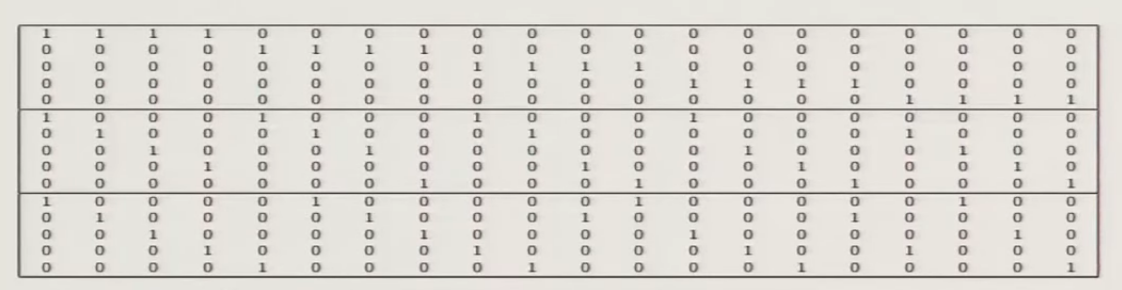
\includegraphics[width=\textwidth]{encoding/R LDPC.png}
		\end{figure}
\end{exampleblock}
Example of Regular Low-density  code matrix; n=20, $w_c$ = 3,  $w_r$ = 4   
\end{frame}

\subsection{Tanner Graphs}
\begin{frame}{Tanner Graphs}
1. A bipartite graph is one in which the nodes can be partitioned into two classes, and no edge can connect nodes from the same class.\\
2. A tanner graph for an LDPC code is an bipartite graph such that:\\
\;\;\;\;\; $\bullet$ One class of the nodes is the "Variable nodes" corresponding to 'n' bits in the code word.\\
\;\;\;\;\; $\bullet$ Second class of nods is "check nodes" corresponding to 'm' parity check equations.\\
\;\;\;\;\; $\bullet$ An edge connects a variable node to the check node if and only if that particular bit is included in the parity check equation.
\end{frame}

\subsection{Gallagher's Construction}
\begin{frame}{Gallagher's Construction for regular (n, $w_c$ , $w_r$) code}

$\bullet$ Let, n be the transmitted block-length of an information sequence of length k. m is the number of parity check equations.\\
$\bullet$ Construct a m $\times$ n matrix with $w_c$ 1's per column and $w_r$ 1's per row.(An (n, $w_c$ , $w_r$)code).\\
$\bullet$ Divide a m$\times$n matrix into $W_c$, m/$W_c$ $\times$n sub-matrices, each containing a single 1 in each column.\\
$\bullet$ The first of these sub-matrices contains all's in descending order.  i.e the $i^{th}$ row contains  's in column(i - 1).$w_r$ + 1 to i.$w_r$.

$\bullet$  The order sub-matrices are merely column permutations of the first sub-matrix.

\end{frame}



